%
% Vorlage für Versuchsprotokolle im Grundpraktikum an der RWTH Aachen
% -------------------------------------------------------------------
%
% Bitte verwenden Sie diese Vorlage zur Erstellung Ihrer
% Protokolle.
%
% Wenn möglich, drucken Sie Ihre Protokolle bitte doppelseitig
% aus. Wenn Sie das Protokoll doppelseitig ausdrucken, verwenden Sie
% die twoside Option ...
\documentclass[twoside]{protokoll}
% ... wenn Sie nicht doppelseitig ausdrucken können, lassen Sie sie
% weg:
%\documentclass{protokoll}
 
% Setzen Sie hier den jeweiligen Versuchsnamen ein:
\versuchsname{Versuchsname}

% Setzen Sie hier Ihre(n) Namen und Ihre Matrikelnummer(n) sowie Ihre
% Gruppennummer ein:
\teilnehmer{Name 1, Matrikelnr}
\teilnehmer{Name 2, Matrikelnr}
\gruppe{Gruppennummer}

\begin{document}

% Hier wird die zum Versuch gehörende Aufgaben ausgewählt, indem das
% Prozentzeichen (%) vor dem entsprechenden \input-Befehl entfernt
% wird. Die tex-Datei kann im Moodle beim jeweiligen Versuch
% heruntergeladen werden. Achten Sie darauf, dass sich alle benötigten
% Dateien im selben Verzeichnis befinden, bevor Sie diese tex-Datei
% kompilieren.
%
% Die Bearbeitung der Aufgaben findet unmittelbar in der jeweiligen
% Datei ("aufgaben_xyz.tex") statt. Dort befinden sich Umgebungen
% der Form
%
% \begin{aufgabe}
%   ... (Aufgabentext) ...
% \end{aufgabe}
%
% Hinter dem versuchsspezifischen Aufgabentext und dem "\end{aufgabe}"
% beginnen Sie jeweils Ihre Lösung der Aufgabe.
%

% Mechanik
%\input{aufgaben_pendel.tex}

% Akustik
%\input{aufgaben_emodul.tex}
%\input{aufgaben_stehende_wellen.tex}

% Thermodynamik
%\input{aufgaben_adiabatenkoeffizient.tex}
%\input{aufgaben_dampfdruckkurve.tex}

% Optik
%\input{aufgaben_prismenspektrometer.tex}
%\input{aufgaben_interferometer.tex}

% Elektrizitätslehre
%\input{aufgaben_lcr_serienschwingkreis.tex}

%
% Der nachfolgende Abschnitt mag nützlich sein, um Vorlagen für häufig
% vorkommende Arbeitsschritte mit LaTeX daraus zu entnehmen. Er muss
% vor Abgabe des Protokolls entfernt werden. (Das \end{document} muss
% aber natürlich erhalten bleiben.)
%
\clearpage
\section*{Grundlagen von \LaTeX}
Hier sollen die wichtigsten Grundlagen von \LaTeX{} knapp rekapituliert
werden, die typischerweise bei der Erstellung eines
Praktikumsprotokolls benötigt werden. Sie können die Beispiele aus
diesem Abschnitt als Vorlage für Ihre eigenen Protokolle
verwenden. Für eine tiefergehende Dokumentation sei auf die Literatur
verwiesen, wobei zu Beginn insbesondere die folgenden Quellen
hilfreich sein können:
\begin{enumerate}
\item T.~Oetiker, Not so short Introduction to \LaTeX,
  \url{www.ctan.org/tex-archive/info/lshort/german/l2kurz.pdf}.
\item Dokumentation, die von der Overleaf-Plattform frei zugänglich
  zur Verfügung gestellt wird: \url{www.overleaf.com/learn}.
\end{enumerate}

\subsection*{Formeln}
Einfache Formeln wie $s=vt$ können direkt im Text gesetzt
werden. Wichtige oder kompliziertere Gleichungen werden mittels einer
\texttt{equation}-Umgebung gesetzt:
\begin{equation}
  \label{eq:fehlerrechnung}
  \left(\frac{\sigma_s}{s}\right)^2 =
  \left(\frac{\sigma_v}{v}\right)^2 +
  \left(\frac{\sigma_t}{t}\right)^2.
\end{equation}
Über Referenzen kann man dann einfach auf die entsprechende
Gleichung~(\ref{eq:fehlerrechnung}) verweisen.

\subsection*{Einheiten}
Um einheitenbehaftete Größen korrekt zu setzen, wird das Paket
\href{https://ctan.org/pkg/siunitx?lang=de}{\texttt{siunitx}}
verwendet. Beispiele finden sich in folgendem Satz: ``Das Pendel hat
eine Länge von \qty{1.5}{m} bei einer Temperatur von
$T=\qty{20}{\degreeCelsius}$. Das führt zu einem Ergebnis von
$g=\qty{9.82+-0.14}{m/s^2}$.''

\subsection*{Abbildungen}
Abbildungen lassen sich mit einer \texttt{figure}-Umgebung
einfügen. Verweise (Abb.~\ref{fig:beispiel}) lassen sich dann
automatisch in den Text einbinden. Wählen Sie für den Export von
Abbildungen das richtige Dateiformat: Für Darstellungen am Bildschirm,
also z.B.~für Vorträge, werden Pixelgrafiken benötigt. Hierfür bietet
sich insbesondere das \texttt{png}-Format an, bei dem die Bilddaten
verlustfrei komprimiert werden. Für Abbildungen im Protokoll
exportiert man die Plots als Vektorgrafik, denn diese lässt sich
beliebig skalieren. Man verwendet am besten das \texttt{pdf}-Format,
weil es sich direkt mit \texttt{pdflatex} verarbeiten
lässt. (\textbf{Ausnahme}: Plots mit sehr vielen Datenpunkten (mehr
als ein paar tausend) bringen unter Umständen den Moodle-Lernraum zum
Absturz und müssen als \texttt{png} abgespeichert werden.) Fotos
u.ä.~können direkt im \texttt{jpg}-Format eingebunden werden. Für
Plots ist das \texttt{jpg}-Format aber keinesfalls geeignet, weil dann
regelmäßig starke Kompressionsartefakte auftreten.
\begin{figure}[t]
  \centering
  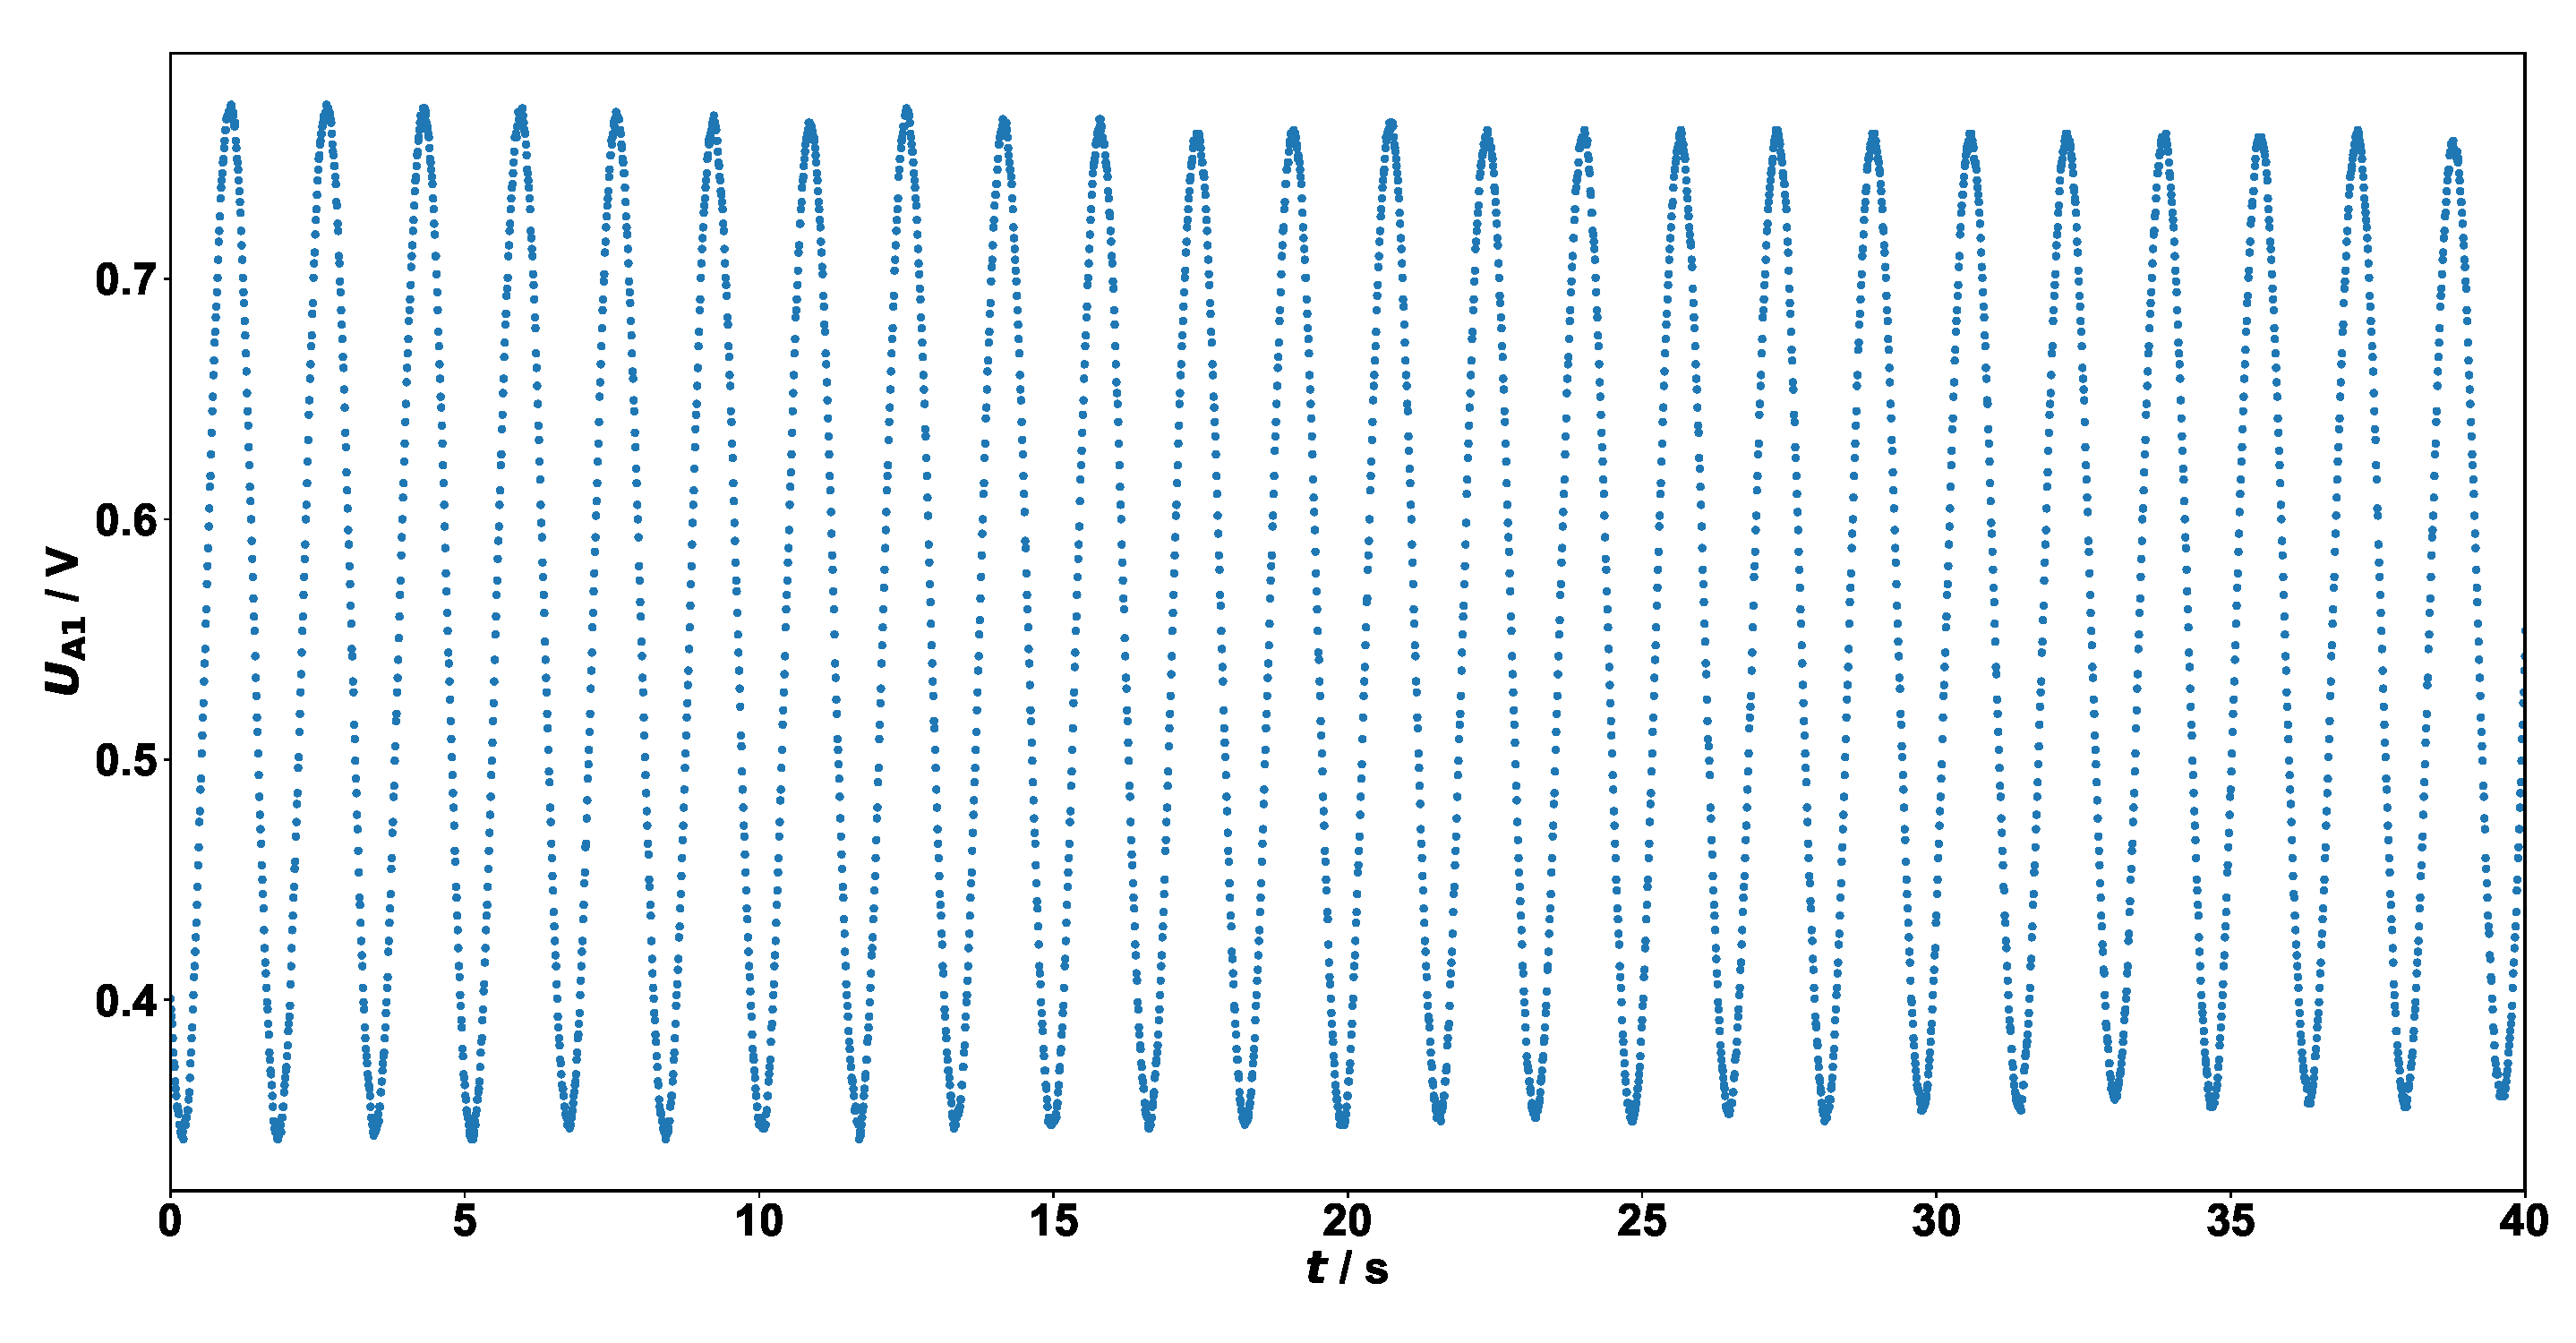
\includegraphics[width=0.95\textwidth]{beispiel_abbildung.pdf}
  \caption{Beispiel für eine Abbildung. In der Bildunterschrift
    sollten alle Informationen enthalten sein, die für das Verständnis
    der Abbildung benötigt werden. Die Interpretation des gezeigten
    findet dann aber im Text statt.}
  \label{fig:beispiel}
\end{figure}

\subsection*{Tabellen}
Tabellen werden mit der \texttt{tabular}-Umgebung gesetzt, die sich
innerhalb einer \texttt{table}-Umgebung befindet, wie im Beispiel von
Tabelle~\ref{tab:beispieltabelle}.
\begin{table}[h]
  \centering
  \begin{tabular}{l|ccc}
    Position $S$ (cm) & \multicolumn{3}{|c}{Laufzeiten $t$ (ms)} \\ \hline
     2,0 & 0,8943 & 0,8944 & 0,8943 \\
         & 0,8953 & 0,8945 & 0,8942 \\ \hline
     6,0 & 0,9921 & 0,9912 & 0,9923 \\
         & 0,9922 & 0,9902 & 0,9929 \\ \hline
    10,0 & 1,0988 & 1,0977 & 1,0982 \\
         & 1,0991 & 1,0992 & 1,0993 \\ \hline
  \end{tabular}
  \caption{Beispieltabelle.}
  \label{tab:beispieltabelle}
\end{table}

\subsection*{Einstellungen}
Um Messwerterfassungseinstellungen und ähnliches kompakt
zusammenzustellen, eignet sich die \texttt{verbatim}-Umgebung:
\begin{verbatim}
Kanal A: Einstellungen
Kanal B: Einstellungen
Messparameter: ...
\end{verbatim}

\subsection*{Protokoll setzen}
Um aus den \LaTeX{}-Quellen eine pdf-Datei zu erzeugen, verwendet man
unter Linux am einfachsten den folgenden Befehl:
\begin{verbatim}
  latexmk -pdf Protokoll
\end{verbatim}

\noindent Dabei ist \texttt{Protokoll} durch den jeweiligen Dateinamen zu
ersetzen, die Endung \texttt{.tex} kann weggelassen werden.

%
% Es folgen Checklisten, mit denen man die häufigsten Fehler bei
% typischen Arbeitsschritten im Praktikum vermeiden kann. Bitte vor
% Abgabe des Protokolls entfernen!
%
\clearpage
\section*{Checklisten}
Es folgen Checklisten, mit denen man die häufigsten Fehler bei
typischen Arbeitsschritten im Praktikum vermeiden kann. Bitte vor
Abgabe des Protokolls entfernen!

\subsection*{Diagramme}
\begin{checklist}
\item Achsenbeschriftungen vollständig mit Größe und Einheit?
\item Wertebereich in $x$- und $y$-Richtung sinnvoll gewählt?
\item Ausreichende Schriftgröße für alle Beschriftungen?
\item Ausreichende Liniendicke, Symbolgröße, etc.?
\item Aussagekräftige Bildunterschrift hinzugefügt?
\item Aussagekräftige Legende, falls notwendig?
\item Abbildung in ausreichender Größe im Protokoll eingebunden?
\item Richtiges Dateiformat gewählt? In aller Regel Vektorgrafik: eps
  oder pdf, \textbf{Ausnahme}: Plots mit sehr vielen Datenpunkten
  (mehr als ein paar tausend), diese bringen unter Umständen den
  Moodle-Lernraum zum Absturz und müssen als png eingebunden werden.
\item Verweis auf Abbildung im Text eingefügt? Auf jede Abbildung muss
  im laufenden Text verwiesen werden.
\end{checklist}

\noindent In aller Regel werden Messdaten in Form von kreisförmigen Markern,
ggfs.~mit Fehlerbalken, eingetragen, Modellanpassungen u.ä.~dagegen in
Form von Linien bzw.~Kurven. Lediglich wenn sehr viele Messpunkte
vorliegen, kann es angemessen sein, statt einzelner Punkte eine alle
Messpunkte verbindende Linie einzuzeichnen.

\subsection*{Regressionsanalyse}
\begin{checklist}
\item Aussagekräftiges Diagramm (s.o.)?
\item Fehler auf Einzelpunkte, in $y$- und ggfs.~in $x$-Richtung
  diskutiert?
\item Diejenige Größe mit den kleineren relativen Unsicherheiten auf
  der $x$-Achse aufgetragen?
\item Residuenplot entsprechend des Beispiels aus der
  Praktikumsbibliothek hinzugefügt und korrekt beschriftet?
\item $\chi^2/dof$ angegeben, und zwar getrennt und im Verhältnis, in
  der Form $\chi^2/dof=24/20=1.2$?
\item Möglicherweise erkennbare systematische Abweichungen von der
  Modellkurve diskutiert?
\end{checklist}

\subsection*{Fourieranalyse}
\begin{checklist}
\item Abtastrate und Dauer der Messung geschickt gewählt?
\item Im Fourierspektrum ggfs.~den Ausschnitt der Frequenzachse so
  angepasst, dass Form und Breite von Peaks gut beurteilt werden
  können?
\item Statistische Messunsicherheit der Peakposition durch
  Wiederholungsmessung bestimmt? Behelfsweise Abschätzung, wie genau
  die Lage des Peaks besimmt werden kann.
\end{checklist}

\subsection*{Ergebnisse}
\begin{checklist}
\item Endergebnisse angegeben und klar als solche kenntlich gemacht?
\item Endergebnisse mit Einheit sowie statistischer und
  ggfs.~systematischer Messunsicherheit angegeben?
\item Nur
  \href{https://de.wikipedia.org/wiki/Signifikante_Stellen}{signifikante
    Stellen} angegeben? Grundsätzlich werden Ergebnis und
  Unsicherheit(en) in derselben Einheit und mit derselben Anzahl an
  Stellen angegeben. Die richtige Anzahl der Stellen wird dabei durch
  die größte Unsicherheit festgelegt. Es gibt zwei Konventionen, die
  man verwenden kann: Entweder man rundet auf zwei signifikante
  Stellen. Oder man folgt der Konvention der Particle Data
  Group\footnote{Abschnitt 5.3 in der
    \href{https://pdg.lbl.gov/2024/reviews/rpp2024-rev-rpp-intro.pdf}{hier
      verlinkten} Einführung.} Letztere ist im \texttt{python}-Modul
  \texttt{uncertainties} implementiert \footnote{Wenn man eine Größe
    als \texttt{ufloat} definiert und sie dann mit \texttt{str} in
    einen String umwandelt bzw.~sie mit \texttt{print} ausgibt, erhält
    man eine korrekt gerundete Darstellung mit genau den signifikanten
    Stellen.}. Eine korrekte Angabe lautet also zum
  Beispiel\footnote{Für den korrekten Textsatz von (fehlerbehafteten)
    Größen mit Einheiten in \LaTeX{} empfiehlt sich dringend die
    Verwendung des \texttt{siunitx} Pakets.}:
  \begin{displaymath}
    g=\qty{9.82+-0.14}{\meter\per\second\squared}.
  \end{displaymath}
\item Vergleich mit Literaturwert oder Herstellerangabe?
\item Ggfs.~Vergleich von Ergebnissen, die mit verschiedenen Methoden
  gewonnen wurden, durchgeführt?
\end{checklist}

\subsection*{Protokollabgabe}
\begin{checklist}
\item Alle Aufgaben bearbeitet?
\item Versuchsdurchführung: Verwenden Sie die 1. Person im Perfekt
  Indikativ (\glqq{}wir haben darauf geachtet\grqq{}, nicht aber
  \glqq{}man sollte darauf achten\grqq{})?
\item Auswertung: Vorgehen nachvollziehbar beschrieben? Verwendete
  Formeln (insbesondere zur Fehlerrechnung) und relevante
  Zwischenergebnisse angegeben?
\item Alle Dateien gemäß der vorgegebenen Konvention benannt?\newline
  D.h.~\texttt{Matrikelnummern\_Versuchsname\_xxx.tex/pdf/py/labx}
  etc., wobei \texttt{xxx} nur aus Buchstaben, Zahlen und
  Unterstrichen bestehen, aber keine Umlaute, Leerzeichen
  usw.~enthalten darf.\newline
  Beispiel:
  \texttt{444444\_445555\_Interferometer\_Protokoll.pdf}.
\item Auswerte-Skripte und Rohdaten abgegeben?
\item Lokale Verzeichnispfade in Skripten entfernt?
\item Testatbogen eingescannt und auch abgegeben?
\item Abgabe final zur Bewertung eingereicht und nicht nur als Entwurf
  gespeichert?
\end{checklist}

% 
% Ende des Protokolls
%
\end{document}
